\documentclass{article}
\usepackage[utf8]{inputenc}
\usepackage{multicol}
\usepackage{enumitem}
\usepackage{amsmath}
\usepackage{graphicx}
\usepackage[compact]{titlesec}
\usepackage{lipsum}
\usepackage[margin=90pt]{geometry}
\usepackage{graphicx}
\usepackage{listings}
\usepackage{color}
\usepackage{flafter}
\usepackage{float}
\usepackage{mathtools}
\usepackage{amsmath}
\usepackage{booktabs}
\usepackage[hang, small,labelfont=bf,up,textfont=it,up]{caption} % Custom captions under/above floats in tables or figures
\geometry{legalpaper, margin=1in}

%%%%%%%%%%%%%%%%%%%%%%%%%%%%%%%%%%%%%%%%%
% Journal Article
% LaTeX Template
% Version 1.4 (15/5/16)
%
% This template has been downloaded from:
% http://www.LaTeXTemplates.com
%
% Original author:
% Frits Wenneker (http://www.howtotex.com) with extensive modifications by
% Vel (vel@LaTeXTemplates.com)
%
% License:
% CC BY-NC-SA 3.0 (http://creativecommons.org/licenses/by-nc-sa/3.0/)
%
%%%%%%%%%%%%%%%%%%%%%%%%%%%%%%%%%%%%%%%%%

%----------------------------------------------------------------------------------------
%	PACKAGES AND OTHER DOCUMENT CONFIGURATIONS
%----------------------------------------------------------------------------------------


%%%%%%%%%%%%%%%%%%%%%%%%%%%%%%%%%%%%%%%%%
% Journal Article
% LaTeX Template
% Version 1.4 (15/5/16)
%
% This template has been downloaded from:
% http://www.LaTeXTemplates.com
%
% Original author:
% Frits Wenneker (http://www.howtotex.com) with extensive modifications by
% Vel (vel@LaTeXTemplates.com)
%
% License:
% CC BY-NC-SA 3.0 (http://creativecommons.org/licenses/by-nc-sa/3.0/)
%
%%%%%%%%%%%%%%%%%%%%%%%%%%%%%%%%%%%%%%%%%

%----------------------------------------------------------------------------------------
%	PACKAGES AND OTHER DOCUMENT CONFIGURATIONS
%----------------------------------------------------------------------------------------

%\documentclass[twoside,twocolumn]{article}

\usepackage{blindtext} % Package to generate dummy text throughout this template 

\usepackage[sc]{mathpazo} % Use the Palatino font
\usepackage[T1]{fontenc} % Use 8-bit encoding that has 256 glyphs
\linespread{1.05} % Line spacing - Palatino needs more space between lines
\usepackage{microtype} % Slightly tweak font spacing for aesthetics

\usepackage[english]{babel} % Language hyphenation and typographical rules


\usepackage{lettrine} % The lettrine is the first enlarged letter at the beginning of the text

\usepackage{enumitem} % Customized lists
\setlist[itemize]{noitemsep} % Make itemize lists more compact

\usepackage{abstract} % Allows abstract customization
\renewcommand{\abstractnamefont}{\normalfont\bfseries} % Set the "Abstract" text to bold
\renewcommand{\abstracttextfont}{\normalfont\small\itshape} % Set the abstract itself to small italic text

\usepackage{titlesec} % Allows customization of titles
\renewcommand\thesection{\Roman{section}} % Roman numerals for the sections
\renewcommand\thesubsection{\roman{subsection}} % roman numerals for subsections
\titleformat{\section}[block]{\large\scshape\centering}{\thesection.}{1em}{} % Change the look of the section titles
\titleformat{\subsection}[block]{\large}{\thesubsection.}{1em}{} % Change the look of the section titles

\usepackage{fancyhdr} % Headers and footers
\pagestyle{fancy} % All pages have headers and footers
\fancyhead{} % Blank out the default header
%\fancyfoot{} % Blank out the default footer
\fancyhead[C]{MALIS final report  $\bullet$ Qlearnkit $\bullet$ Fall 2021 } % Custom header text

\usepackage{titling} % Customizing the title section

\usepackage{hyperref} % For hyperlinks in the PDF

%----------------------------------------------------------------------------------------
%	TITLE SECTION
%----------------------------------------------------------------------------------------

\setlength{\droptitle}{-4\baselineskip} % Move the title up

\pretitle{
\begin{center}\Huge\bfseries} % Article title formatting
\posttitle{\end{center}} % Article title closing formatting
\title{Qlearnkit: a Python toolkit for quantum machine learning} % Article title
\author{%
\textsc{Giulio Corallo, Massimiliano Pronesti, Federico Tiblias}\\
\normalsize Institut EURECOM \\ % Your institution
}
\date{\today} % Leave empty to omit a date
\renewcommand{\maketitlehookd}{%
\begin{abstract}
\noindent Quantum hardware offers new interesting possibilities for training machine learning models given its significant speedup. Plenty of quantum algorithms exist in theory but actual implementation are few and far between. In this paper we describe a possible implementation of the K-NN, K-Means, SVM and Ridge Regression models using quantum circuits. This cohesive implementation is based on Qiskit and collected inside a Python package named Qlearnkit. We have shown that these models perform well in terms of accuracy and various other metrics compared to classical counterparts. Time performances on the other hand were relatively low since simulating quantum hardware adds a significant computation overhead.
\end{abstract}
}

%----------------------------------------------------------------------------------------
%------------------------------------------------
%% Bibliography

\usepackage[sorting=none, backend=bibtex]{biblatex}
\addbibresource{ref.bib}

\begin{document}
% Print the title
\maketitle
%----------------------------------------------------------------------------------------
%	ARTICLE CONTENTS
%----------------------------------------------------------------------------------------




\begin{multicols}{2}
\section {Introduction}\lettrine[nindent=0em,lines=3]{M}achine learning and deep learning techniques are gaining more and more attention given the breakthrough results of recent years \cite{Vaswani2017-lk} \cite{NIPS2012_c399862d}. Nonetheless, the ever-increasing complexity of such models is growing side by side with the computational resources needed to train them. This led researchers to investigate further computational solutions \cite{Buffoni2021-jg}. Among the many promising alternatives, quantum computing  stands out, given its potential in terms of execution speedup for large-scale problems. In fact, it has been shown that quantum algorithms exhibit rather significant speedups in commonly used subroutines such as Fourier transforms, finding eigenvectors and eigenvalues, solving linear equations, some even attaining an exponential advantage over their classical counterparts. These speedups translate very well into an increase in performance for commonly used techniques in machine learning and convex optimization such as Principal Component Analysis, kernel methods, Support Vector Machines, least-squares fitting and gradient descent \cite{Biamonte2016-rb}.  In this paper we describe our implementation of the following well-known supervised and unsupervised machine learning algorithms for a gated quantum computer: Least-Squares Support Vector Machine, K-Nearest Neighbors, K-Means clustering and Ridge Regression. These implementations have been assembled into a Python library named qlearnkit, built on top of Qiskit and available on \href{https://github.com/mspronesti/qlearnkit}{GitHub} and \href{https://pypi.org/project/qlearnkit}{PyPI}.



\section{Related Work}
Building a proper, physically scalable and stable quantum computer is a rather difficult task. Nevertheless, research in the field and its application to different domains, such as cryptography and machine learning has been carried out since the late '80s, providing theoretical implementations and insights on their benefits with respect to the classical versions. An excellent summary of near future quantum computing applications to machine learning is provided in \cite{phillipson}, where the authors show how purely quantum or hybrid version of machine learning techniques can perform better in several directions, such as runtime, capacity or learning itself.
\cite{zhang} provides insights into the state-of-the-art quantum machine learning implementations. In section 4, it is pointed out that quantum computing will be able to speedup learning techniques in different degrees, since the subroutines such as HHL and amplitude amplification can provide exponential speedup and quadratic speedup separately, e.g. exponential speedup to Quantum LDA, Quantum PCA and Quantum SVM, Quadratic speedup to Quantum K-Means clustering.

From the software point of view, being quantum machine learning a nascent field, not many toolkits exist in the market or among the open-source community. Qiskit (\cite{Qiskit}) and IBM are definitely  leading the path and qiskit-machine-learning, born from the now deprecated qiskit-aqua, provides some pure and hybrid quantum machine learning implementations. Differently from Qiskit, qlearnkit looks at the ease of usage and implements different classification, regression and clustering techniques.

Another relevant work is Pennylane (\cite{Pennylane}), a cross-platform Python library for differentiable programming of quantum computers, providing tools for quantum computing and machine learning though offering a different approach towards usage. In fact, it seamlessly integrates classical machine learning libraries with quantum simulators and hardware, giving users the power to train quantum circuits. 

Finally, \cite{qknn} is a fancy implementation of a pure quantum K-Nearest-Neighbors classifier built on top of qiskit and developed as a work of thesis at Radboud University Nijmegen in collaboration with ING Quantum Technology. Differently from it, qlearnkit employs a simpler quantum architecture and reduces the constraints on the number of required qubits, the speed of execution and avoids race conditions appearing due to an incorrect use of parallelization with bigger datasets, where [6] seems to fail.

\section{Datasets}
The Datasets we used to test our implementations of the quantum algorithms are those provided by scikit-learn\cite{sklearn_api}, in particular iris, wine, diabetes,  make\_regression, make\_classification and make\_blobs.


The Results section clarifies which datasets are used on which models.
\section{Methods}
\subsection{Quantum Encodings}
Quantum computers expect data in quantum state for processing. The first step in quantum machine learning is to load classical data by encoding it into the state of the qubits. This process is also known as quantum data encoding \cite{data_encoding} or embedding and is an important step in Quantum state preparation. Classical data encoding for quantum computation plays a critical role in the overall design and performance of the quantum machine learning algorithm. 


In the specific case of our library, we implemented amplitude and angle encodings.
Amplitude encoding represents classical data as amplitudes of quantum states.
Angle encoding, contrarily, represents classical features as angles of a multi-qubit system.

\subsection{Quantum K-Nearest Neighbors}
The quantum version of the K-Nearest Neighbors algorithm estimates the distance of two vectors in the following way:
given a zero initialized ancillary qubit and a quantum state \(\lvert \Psi\rangle\) which stores vectors we want to estimate
$$ \lvert 0\rangle\lvert\Psi\rangle , \lvert \Psi\rangle = \lvert \psi \rangle\lvert \phi \rangle$$
First we apply a Hadamard gate to the ancillary qubit, pushing it into superposition
$$ \frac{1}{\sqrt{2}}(\lvert 0\rangle + \lvert 1\rangle)\lvert \Psi\rangle $$
To entangle the state \(\Psi\) with our ancillary qubit, we apply a swap gate to \(\Psi\) controlled on the ancillary qubit
$$ \frac{1}{\sqrt{2}}(\lvert 0\rangle \lvert \Psi\rangle + \lvert 1\rangle F(\lvert \Psi\rangle))\lvert \Psi\rangle $$
where \(F(\lvert \Psi\rangle)\) represent the swapped version of \(\lvert \Psi\rangle\)
$$F(\lvert \Psi\rangle) = \lvert \phi\rangle \lvert \psi\rangle $$
Finally we apply another Hadamard gate to the ancillary qubit
$$ \frac{1}{2}(\lvert 0\rangle \lvert (I + F)\Psi\rangle + \lvert 1\rangle \lvert(I - F)\Psi\rangle) $$
where $I$ is the identity operator.
Thus, the probability of the ancillary qubit being measured as in the \(\lvert 1\rangle\) state is 
$$ P(\lvert 1\rangle) = \lvert \Psi\rangle \frac{I-F}{2} \lvert \Psi\rangle = \langle \psi\phi\lvert \frac{I-F}{2} \lvert \psi\phi\rangle $$
Expanding the inner product we get
$$ P(\lvert 1\rangle) = \frac{1}{2}\langle \psi\phi, (\lvert \psi\phi\rangle - \lvert \psi\phi \rangle) \rangle  = \frac{1 - \langle \psi, \phi \rangle ^2}{2}$$
The last term is proportional to the square distance between two normalized vectors.
This proves rather interesting from a quantum point of view as we exploit an inner property of states in quantum mechanics instead of directly measuring it \cite{Basheer2020-ww}. This approach, called SWAP test, is the key for the quantum distance measurement.
\begin{figure}[H]
  \centering
    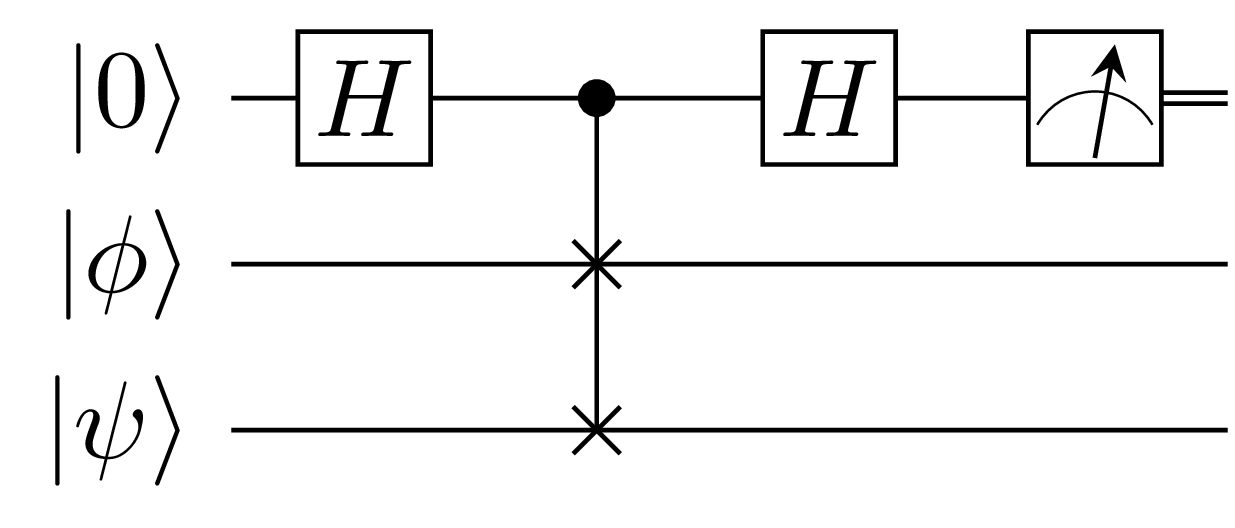
\includegraphics[width=.8\linewidth]{assets/kmeans/Quantum-swap-test-circuit-correct.png}
    \caption{Swap Test Circuit}
\end{figure}
There are other explorable metrics proposed in scientific literature, such as the Hamming distance metric \cite{Li2021-le}, nevertheless the first one sticks to the traditional idea of the classical K-NN algorithm. In fact, after constructing the quantum circuits, their results are used to compute the fidelities and eventually to do a majority voting to predict the class. 

\subsection{Quantum K-Means}
In a classical K-Means algorithm, given a dataset, at each iteration, the data points are assigned to a cluster according to the Euclidean distance. The centroids are then updated so that the new centroid is the average of all points that have been assigned to the cluster in this iteration. The loss function that this algorithm is trying to minimize is the RSS (residual sums of squares). A single iteration has complexity of $O(kNd)$ and the algorithm can be super-polynomial in the worst case \cite{10.1145/1137856.1137880}.
The quantum version of the K-Means algorithm has performance similar to the classical K-Means and provides a running time with substantial savings, especially for large datasets, in fact the running time is poly-logarithmic in the number of elements of the dataset \cite{Kerenidis2018-gl}.
In order to run the QKMeans algorithm we firstly map data feature values to a quantum state:
\begin{align*}
\phi = \frac{(x+1)\pi}{2}\\
\theta = \frac{(x+1)\pi}{2}
\end{align*}
(where \(\phi\) is the phase and \(\theta\) the angle) and then we perform encoding using the U gate provided by the Qiskit library.
The algorithm is then run with a similar logic to the classical one. First, we pick some random initial points using some heuristic, for example K-Means++\cite{10.5555/1283383.1283494}. At each step of our iteration, we need to compute distances of our new data point with respect to the centroids of our cluster, which is easily doable in a quantum context, in a similar way as explained for the Quantum K-NN. Alternatively, instead of constructing a 1-level SWAP test circuit we can construct a $k$-level circuit, where $k$ is the number of clusters, in order to compute in one-shot the distances of a state vector with respect to the $k$ cluster centroids. This can get better performances and high parallelism. Below a figure of the circuit assuming $k=3$.
\begin{figure}[H]
  \centering
    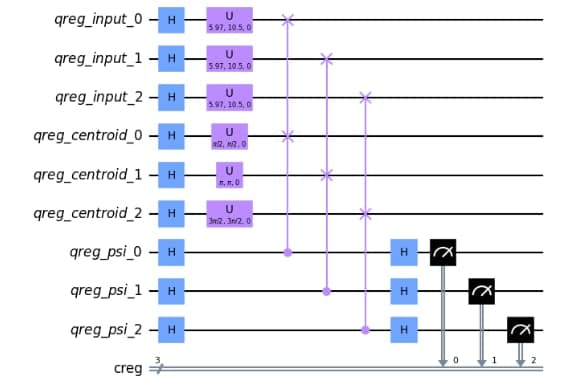
\includegraphics[width=\linewidth]{assets/kmeans/qkmeans_circuit.jpg}
\end{figure}

However, in this case the number of qubit needed increases. In fact, for each level added, we need 3 more qubits.

\subsection{Quantum Support Vector Machines}
Quantum SVMs offer an exponential speedup in training and predicting compared to classical ones. An SVM convex optimization problem can be reformulated into a system of linear equations in the form \(Ax= b\), the solution of which is a trained SVM model:
\begin{align*}
\begin{bmatrix}
0 & 1^T_M \\
1_M & K+\gamma^{-1}I_M 
\end{bmatrix}
\begin{bmatrix}
\beta \\
\alpha
\end{bmatrix} = 
\begin{bmatrix}
0 \\
Y
\end{bmatrix}
\end{align*}
with $M$ number of training samples, $K=K(x_i,x_j)$ kernel matrix, $X$ training set, $Y$ classification labels, $\gamma$ regularization hyperparameter, $1_M = [1,...1]^T$, $I_M$ identity matrix, $\alpha$ and $\beta$ respectively weights and bias used in prediction.
Model prediction on new data can be obtained as
\begin{align*}
f(\cdot) = K( \cdot,X) \cdot \alpha + \beta
\end{align*}

Building $A$ requires computing the kernel matrix $K$ of distances from each sample to each sample, and solving the system requires a matrix inversion \cite{svm_inversion}. The kernel matrix can be obtained exponentially faster using quantum computers: a kernel function can be evaluated with a \(O(log N)\) complexity against the \(O(N)\) of classical computers, where N is the number of features \cite{Rebentrost2013-ar}.
Taking advantage of these two properties, we implemented an algorithm capable of constructing a kernel matrix and computing the solution of a linear system in time \(O(M^3+ M^2 log N)\) \cite{Havlicek2018-hi}. First we build the kernel matrix using Qiskit’s FeatureMaps, then we prepare the \(Ax = b\) system and finally we solve it with a matrix inversion. A further refined version of the algorithm was formulated that can enhance the matrix inversion and provide a total runtime of \(O(log MN)\). However, it was not implemented due to time and complexity constraints.

\subsection{Quantum Kernel Ridge Regression}
We know a closed-form solution of the Ridge Regression problem exists that requires computing a kernel matrix of points \cite{lecture_6}. In a way almost identical to the Quantum SVM described above, we start 
from the linear system formulation of the problem but delegate the computing of the kernel matrix to a quantum subroutine, thus obtaining a speedup.
\section{Results}
\subsection{Quantum K-Nearest Neighbors}
The Quantum K-Nearest Neighbors Classifier was compared against a classical version employing the euclidean metric for distance measurement, in terms of accuracy, F1-score and Jaccard index. The plots below were generated training the models using $k = 3$ and the full Iris dataset normalized via amplitude encoding. The classical data has been reduced via PCA with 2 components before plotting the results.

Both the qasm\_simulator and the statevector\_simulator provided by Qiskit produce the same results, classifying the data well enough with respect to the classical version provided by scikit-learn. It should be noted, however, that in this example the classification process was affected by the precision of the measurement.

\begin{figure}[H]
  \centering
    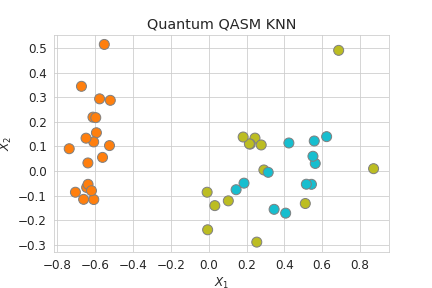
\includegraphics[width=\linewidth]{assets/knn/Quantum QASM KNN.png}
    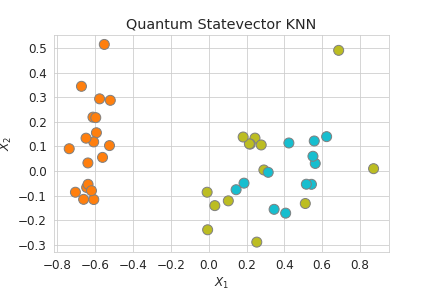
\includegraphics[width=\linewidth]{assets/knn/Quantum Statevector KNN.png}
    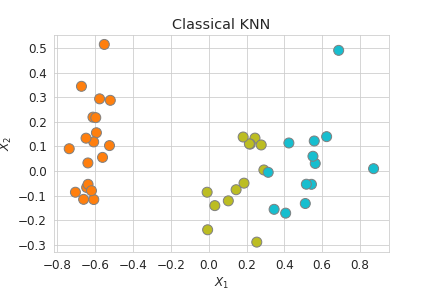
\includegraphics[width=\linewidth]{assets/knn/Classical KNN.png}
    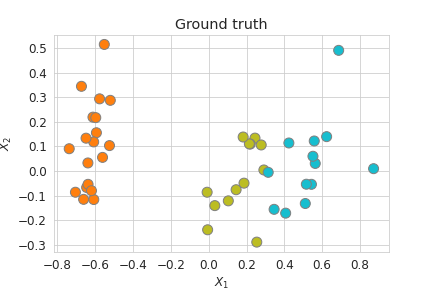
\includegraphics[width=\linewidth]{assets/knn/gt.png}
\end{figure}

\captionof{table}{K-NN performance results}
\begin{center}
\begin{tabular}{lccccl}
\toprule
  & ACC    & F1  & JAC  \\
  \midrule
 QASM K-NN & 0.930 & 0.930 & 0.850    \\
 Statevector K-NN  & 0.930 & 0.930 & 0.850    \\
 Classical K-NN & 1.000 & 1.000 & 1.000   \\
\bottomrule
\end{tabular}
\end{center}


\subsection{Quantum K-Means}
The Quantum K-Means clustering was tested on a synthetic dataset generated using scikit-learn's make\_blobs. make\_blobs generates isotropic Gaussian blobs for clustering. From this data we rescaled each feature into the $[0, 1]$ range. We tested the algorithm with both a noisy and a non-noisy backend, respectively qasm\_simulator and statevector\_simulator.


\begin{figure}[H]
  \centering
    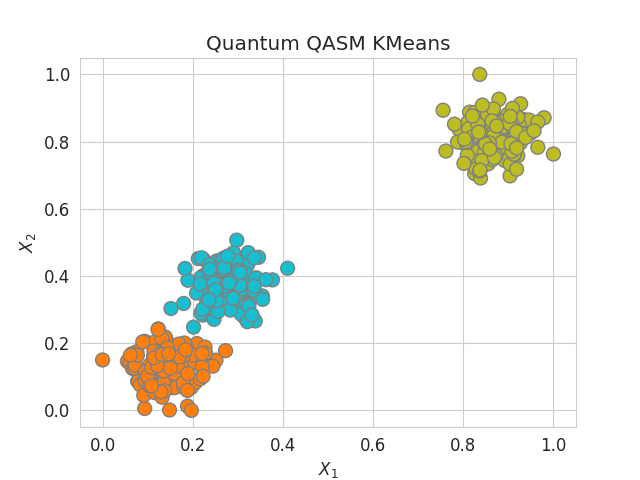
\includegraphics[width=\linewidth]{assets/kmeans/Quantum QASM KMeans.png}
    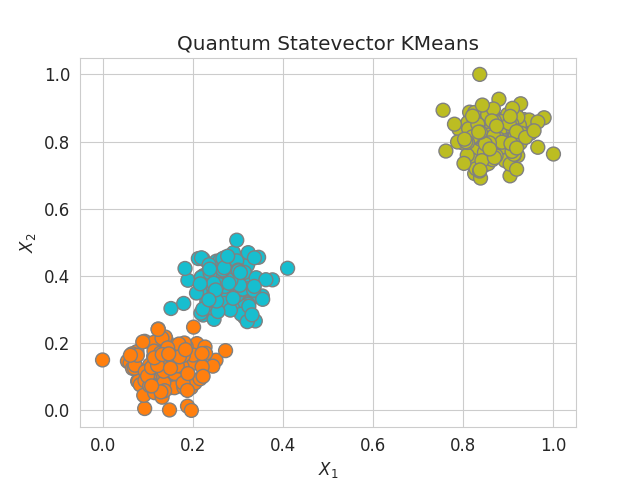
\includegraphics[width=\linewidth]{assets/kmeans/Quantum Statevector KMeans.png}
  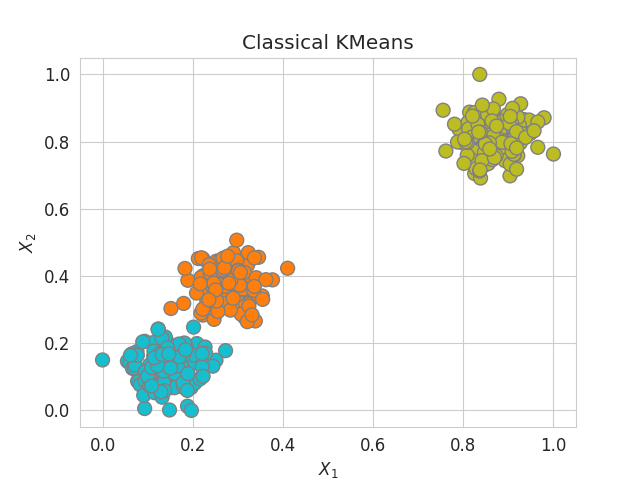
\includegraphics[width=\linewidth]{assets/kmeans/Classical KMeans.png}
    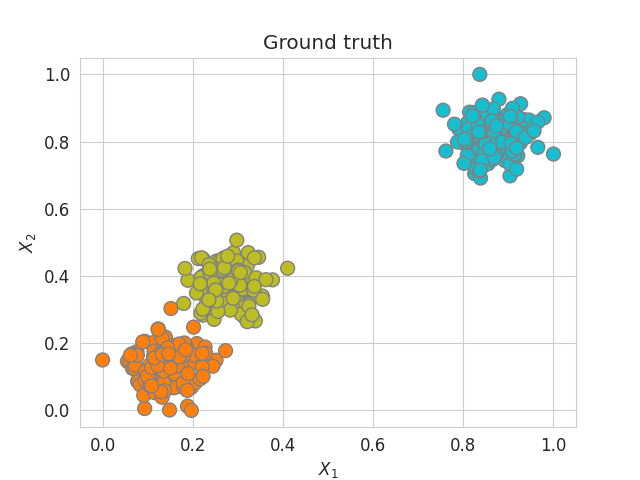
\includegraphics[width=\linewidth]{assets/kmeans/gt.png}
\end{figure}


On top of the Silhouette score, we evaluated the performance of Quantum K-Means using Adjusted Rand Index and Completeness. The results of this analysis are shown in Table 3. More detailed informations can be found in \cite{metrics}.

\captionof{table}{KMeans performance results}
\begin{center}
\begin{tabular}{lcccl}
\toprule
     &  SIL & ARI & COMP\\
     \midrule
     QASM K-Means & 0.747 & 0.978 & 0.968\\
     Statevector K-Means & 0.750 & 0.993 & 0.987\\
     Classical K-Means & 0.750 & 0.993 & 0.987 \\
     \bottomrule
    \end{tabular}
    \end{center}
    


    Our simulations shows that Quantum K-Means achieves very similar clusters to those of the classical K-Means algorithm.
In particular, using a non-noisy backend, the Quantum K-Means achieves the exact same clusters of its classical counterpart.

Even using different dataset, such as Iris and Wine, we got similar results.


\subsection{Quantum Support Vector Machines}
Quantum SVM was compared against a classical RBF SVM in terms of accuracy, F1-score and Jaccard index. The synthetic dataset used for this comparison was generated with scikit-learn's make\_classification method, with each feature rescaled into the $[0,1]$ range. 
\begin{figure}[H]
  \centering
    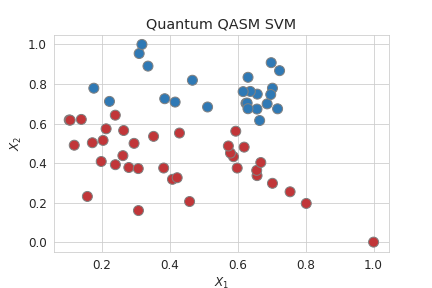
\includegraphics[width=\linewidth]{assets/svm/Quantum QASM SVM.png}
    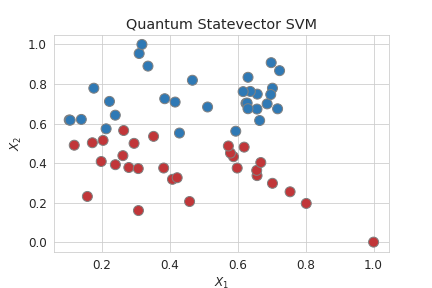
\includegraphics[width=\linewidth]{assets/svm/Quantum Statevector SVM.png}
    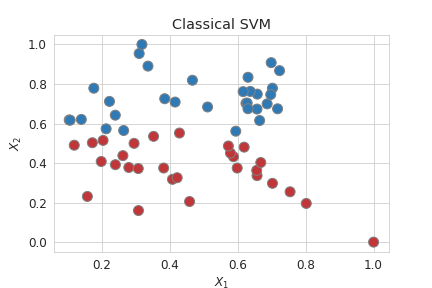
\includegraphics[width=\linewidth]{assets/svm/Classical SVM.png}
    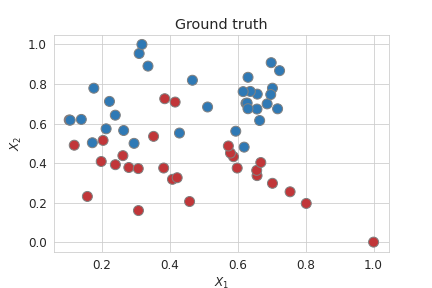
\includegraphics[width=\linewidth]{assets/svm/gt.png}
\end{figure}
Using the qasm\_simulator provided by Qiskit, the quantum model was able to fit the data well enough, correctly identifying the curved decision boundary and assigning the right label to most of the data. Plenty of classification errors can be attributed to the noisy nature of said simulator. By comparison, a non-noisy backend such as statevector\_simulator was able to obtain results almost identical to the classical SVM. Another example of how important noise reduction will be in the development of future quantum computers.

\captionof{table}{SVM performance results}
\begin{center}
\begin{tabular}{lccccl}
\toprule
  & ACC    & F1  & JAC  \\
  \midrule
 QASM SVM & 0.800 & 0.786 & 0.647    \\
 Statevector SVM & 0.883 & 0.889 & 0.800    \\
 Classical SVM & 0.883 & 0.889 & 0.800   \\
\bottomrule
\end{tabular}
\end{center}

\subsection{Quantum Kernel Ridge Regression}
Regression was tested on a synthetic dataset generated using scikit-learn's make\_regression. The quantum model attained an high $R^2$ score, while was greatly outperformed by a classical one in terms of Mean Squared Error. The noise introduced by the qasm\_simulator used is clearly visible and has skewed the results. statevector\_simulator appears smoother. It's also worth noting that the kernel we chose, Qiskit's ZFeatureMap, is non-linear in nature while the data we tried to fit was. We preferred not to design an ad-hoc nonlinear dataset in order to show the interesting properties of quantum feature maps. We believe such an algorithm could still be employed successfully given efficient noise reduction and a suitable dataset.

\begin{figure}[H]
  \centering
    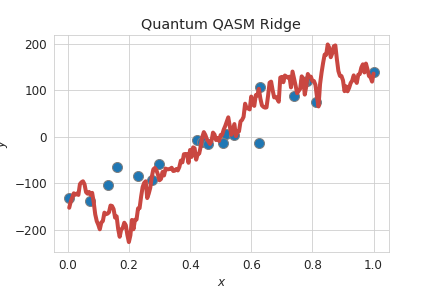
\includegraphics[width=\linewidth]{assets/ridge/Quantum QASM Ridge.png}
  \centering
    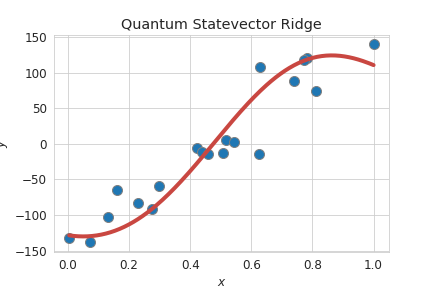
\includegraphics[width=\linewidth]{assets/ridge/Quantum Statevector Ridge.png}
  \centering
    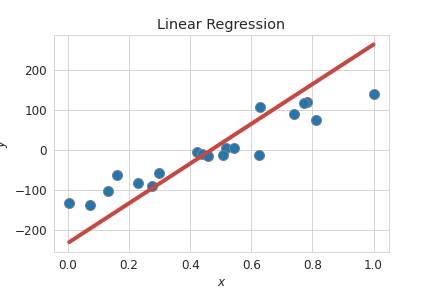
\includegraphics[width=\linewidth]{assets/ridge/Linear Regression.png}
\end{figure}

\columnbreak

\captionof{table}{Ridge performance results}
\begin{center}
\begin{tabular}{lcccl}
\toprule
       & MSE    & $R^2$ \\
\midrule
 QASM Ridge & $4.999*10^{2}$ & 0.930    \\
  Statevector Ridge & $4.265*10^{2}$ & 0.940    \\
 Linear Regression & $1.375*10^{-27}$ & 1.000 \\
\bottomrule
\end{tabular}
\end{center}


\section{Conclusion}
We showed that quantum-based algorithms can compete against optimized well-established classical ones in terms of accuracy. With the notable exception of Qiskit, no cohesive work exists that groups in a familiar and ready-to-use way quantum-based learning algorithms. Running our models on Qiskit proved efficient albeit limiting: as expected, simulating a quantum system requires a significant amount of overhead computation. This prevented our work from competing against classical algorithms in terms of execution time. It’s also worth noting that the scope of our work was bound by the total number of qubits made available by simulators. Qlearnkit can be expanded with other algorithms for which a quantum formulation exists. NNs, PCA and Linear Regression are good candidates, as well as the more efficient SVM formulation mentioned above. An alternative to LS-SVM based on variational circuits is also being considered. 


\section{Contributions}
\textbf{Giulio Corallo}: Quantum K-Means, testing \\\\
\textbf{Massimiliano Pronesti} Quantum K-Nearest Neighbors Classifier and Regressor, repository management, continuous integration and deployment, documentation, testing \\\\
\textbf{Federico Tiblias}: Quantum Support Vector Classifier, Quantum Kernel Ridge Regressor, testing, data visualization\\\\

\end{multicols}
\newpage
\printbibliography

\end{document}

